\documentclass[usenames,dvipsnames, 9pt]{beamer}
\usepackage{amsmath,amsfonts,amssymb}
\usepackage{mathtools}
\usepackage{etex} %for Windows
\usepackage[utf8]{inputenc}
\usepackage[english, russian]{babel} 
%\usepackage{microtype}			% Better interword spacing and additional kerning.
\usepackage{ellipsis}			% Adjusted space with \dots between two words.
\usepackage{graphicx}
\usepackage{pstricks}

\usepackage{xcolor}


\usepackage{changepage}

\usepackage{algorithm}
\usepackage{algpseudocode}
%\usepackage[]{algorithm2e}
%\usepackage{algorithmic}

%\usepackage{tcolorbox}


\usepackage{caption}
\usepackage{subcaption}
%\usepackage{stackengine}


\usepackage{tikz}
\usetikzlibrary{tikzmark,calc}
\usetikzlibrary{positioning, backgrounds}
\usetikzlibrary{arrows, chains, matrix, scopes, patterns, shapes, fit}
\usetikzlibrary{mindmap,trees,shadows}
\usetikzlibrary{decorations.pathreplacing}
%\usetikzlibrary{crypto.symbols}

\usepackage{pgfplots}

\pgfmathdeclarefunction{gauss}{2}{%
	\pgfmathparse{1/(#2*sqrt(2*pi))*exp(-((x-#1)^2)/(2*#2^2))}%
}


\tikzset{
	invisible/.style={opacity=0},
	visible on/.style={alt={#1{}{invisible}}},
	alt/.code args={<#1>#2#3}{%
		\alt<#1>{\pgfkeysalso{#2}}{\pgfkeysalso{#3}} % \pgfkeysalso doesn't change the path
	},
}

\newcommand\strikeout[2][]{%
	\begin{tabular}[b]{@{}c@{}} 
		\makebox(0,0)[cb]{{#1}} \\[-0.2\normalbaselineskip]
		\rlap{\color{Orange}\rule[0.5ex]{\widthof{#2}}{1.5pt}}#2
\end{tabular}}

\newcommand\Fontvi{\fontsize{11}{13.2}\selectfont}

\usepackage{listings} % for C++ code

\usepackage{braket}
%\usepackage[braket, qm]{qcircuit}



\usepackage[T1]{fontenc}
%\usepackage[sfdefault,scaled=.85]{FiraSans}
%\usepackage{newtxsf}
%\usepackage[nomap]{FiraMono}





\usefonttheme[onlymath]{serif}
\renewcommand\sfdefault{cmbr}

\renewcommand{\bfdefault}{sb}

\definecolor{CharCoalDark}{RGB}{13, 16, 19}
\definecolor{Orange}{RGB}{255, 165,0}
\definecolor{DarkOrange}{RGB}{255, 165,0}
\definecolor{LightSalmon}{RGB}{255, 160, 122}
\definecolor{LeafGreen}{RGB}{34, 139,  34}
\definecolor{Coral}{RGB}{255, 127, 80}
\definecolor{DarkTurquoise}{RGB}{0, 206, 209}

%\newtheorem{defRus}{Определение}
%\newtheorem{thmRus}{Теорема}
%s\newtheorem{corRus}{Следствие}


\setbeamercolor{background canvas}{bg=CharCoalDark}

\setbeamerfont{title}{series=\bfseries}
\setbeamercolor{title}{fg=Orange}
\setbeamercolor{section in toc}{fg=white}
\setbeamercolor{frametitle}{fg=Orange}
\setbeamercolor{normal text}{fg=white}
%\setbeamercolor{normal text}{fontsize=12pt}
\setbeamercolor{itemize item}{fg=Orange}
\setbeamercolor{enumerate item}{fg=Orange}
\setbeamercolor{enumerate item item}{fg=Orange}
\setbeamercolor{itemize item item}{fg=Orange}
\setbeamercolor{enumerate item}{fg=Orange}
\setbeamercolor{block title}{bg=DarkOrange,fg=white}
\setbeamerfont{block title}{series=\bfseries}

\setbeamertemplate{itemize item}[circle]
\setbeamertemplate{eumerate subitem}{\color{Orange}[$\checkmark$]}
\setbeamertemplate{itemize subitem}{\color{Orange}\Large$\textbullet$}
\setbeamertemplate{itemize subitem}{\color{Orange} \tiny $\blacksquare$}

% footnote without a marker
\newcommand\blfootnote[1]{%
	\begingroup
	\renewcommand\footnoterule{}
	\renewcommand\thefootnote{}\footnote{#1}%
	\addtocounter{footnote}{-1}%
	\endgroup
}

\newcommand*{\Scale}[2][4]{\scalebox{#1}{\ensuremath{#2}}}%

\newcommand\Item[1][]{%
	\ifx\relax#1\relax  \item \else \item[#1] \fi
	\abovedisplayskip=0pt\abovedisplayshortskip=0pt~\vspace*{-\baselineskip}}

\pgfdeclareradialshading{ring}{\pgfpoint{0cm}{0cm}}%
{rgb(0cm)=(1,1,1);
	rgb(0.7cm)=(1,1,1);
	rgb(0.719cm)=(1,1,1);
	rgb(0.72cm)=(0.975,0,0);
	rgb(0.9cm)=(1,1,1)}

\usepackage[absolute,overlay]{textpos} %to clip to a corner
\newcommand\FrameText[1]{%
	\begin{textblock*}{\paperwidth}(\textwidth-35pt, 10 pt)
		\raggedright #1\hspace{.5em}
\end{textblock*}}

\makeatletter
\let\save@measuring@true\measuring@true
\def\measuring@true{%
	\save@measuring@true
	\def\beamer@sortzero##1{\beamer@ifnextcharospec{\beamer@sortzeroread{##1}}{}}%
	\def\beamer@sortzeroread##1<##2>{}%
	\def\beamer@finalnospec{}%
}
\makeatother

\AtBeginSection[]
{
	\begin{frame}<beamer>
		\frametitle{Outline}
		\tableofcontents[currentsection]
	\end{frame}
}


%\institute{ENS Lyon}
\author{Elena Kirshanova \\ [10pt]
}
\titlegraphic{
	
	%\includegraphics[width=2.5cm]{erc_logo_gray}\hspace*{2.5cm}~%
	%\includegraphics[width=4.0cm]{ens_logo_gray}
}
\title{\Huge Message Authentication Code}

\date{ Course ``Information and Network Security'' \\ 	
	Lecture 5 \\ \today }


\setbeamertemplate{navigation symbols}{} %removes navigation

% proper highlightling of a code-snippet
\lstset{language=C++,
	keywordstyle=\color{magenta},
	stringstyle=\color{Goldenrod},
	commentstyle=\color{gray},
	breaklines=false,
	%morecomment=[l][\color{magenta}]{\#}
}

%\setlength{\parskip}{8pt}
% ==================================================================
% Definitions for this paper
% ==================================================================
\mathchardef\hyphen="2D

\usepackage{multirow}
\usepackage{multicol} % For multiple coloumn environments
%\usepackage{stmaryrd} % For set brackets
% \setlength{\columnsep}{15pt} % Defining the coloumn seperation
% \setlength{\columnseprule}{1pt} % Place a line between coloumns
% \newcommand{\tab}{\hspace*{2em}}

%subscripts

\newcommand*\SmallTextScript[2]{{\mathchoice{\displaystyle #2}
		{\textstyle #2}%dito
		{\scalebox{#1}{\ensuremath{\scriptstyle #2}}}%
		{\scalebox{#1}{\ensuremath{\scriptscriptstyle #2}}}%
}}


% ADVERSARIES AND SUCH
\newcommand*{\poly}{\ensuremath{\mathrm{poly}}}
\newcommand*{\eps}{\ensuremath{\varepsilon}}
\newcommand*{\alg}{\ensuremath{\mathcal{A}}}

% GROUPS/DISTRIBUTIONS/SETS/LISTS
\newcommand{\N}{{{\mathbb N}}}
\newcommand{\Z}{{{\mathbb Z}}}
\newcommand*{\IZ}{\ensuremath{\mathbb{Z}}}
\newcommand*{\IN}{\ensuremath{\mathbb{N}}}
\newcommand*{\IQ}{\ensuremath{\mathbb{Q}}}
\newcommand{\R}{{{\mathbb R}}}
\newcommand*{\IR}{{{\mathbb R}}}
\newcommand{\Zp}{\Z_p} % Integers modulo p
\newcommand{\Zq}{\Z_qs} % Integers modulo q
\newcommand{\Zn}{\ints_N} % Integers modulo N
\newcommand{\F}{\ensuremath{\mathbb{F}}}
\newcommand{\CC}{\ensuremath{\mathbb{C}}}

\newcommand{\ord}{\ensuremath{\mathrm{ord}}}

\newcommand{\GF}{\ensuremath{\mathbb{F}_2}}
\newcommand{\GFn}{\ensuremath{\mathbb{F}^n_2}}

%%% ALGORITHMS/PROCEDURES %%%
\newcommand{\Dec}{\textsf{Dec}}
\newcommand{\Enc}{\textsf{Enc}}
\newcommand{\KeyGen}{\textsf{KeyGen}}
\newcommand{\Gen}{\textsf{Gen}}
\newcommand{\MAC}{\textsf{MAC}}
\newcommand{\sk}{\textsf{sk}}
\newcommand{\pk}{\textsf{pk}}
\newcommand{\mesS}{\ensuremath{\mathcal{M}}}
\newcommand{\keyS}{\ensuremath{\mathcal{K}}}
\newcommand{\cipS}{\ensuremath{\mathcal{C}}}
\newcommand{\tagS}{\ensuremath{\mathcal{T}}}
\newcommand{\nonceS}{\ensuremath{\mathcal{N}}}
\newcommand{\mactag}{\textsf{tag}}
\newcommand{\Hash}{\ensuremath{\mathcal{H}}}
\newcommand{\EID}{\ensuremath{\mathtt{EphID}}}

\newcommand{\rem}{\ensuremath{\mathrm{rem}}}

\newcommand{\adv}{\ensuremath{\mathcal{A}}}

\newcommand{\LWE}{\mathsf{LWE}}
\newcommand{\DCP}{\mathsf{DCP}}
\newcommand{\EDCP}{\mathsf{EDCP}}
\newcommand{\UEDCP}{\mathsf{U \text{-} EDCP}}
\newcommand{\GEDCP}{\mathsf{G \text{-} EDCP}}



%% Landau and proba
\newcommand{\bigO}{\mathcal{O}}
\newcommand*{\OLandau}{\bigO}
\newcommand*{\WLandau}{\Omega}
\newcommand*{\xOLandau}{\widetilde{\OLandau}}
\newcommand*{\xWLandau}{\widetilde{\WLandau}}
\newcommand*{\TLandau}{\Theta}
\newcommand*{\xTLandau}{\widetilde{\TLandau}}
\newcommand{\smallo}{o} %technically, an omicron
\newcommand{\wLandau}{\omega}
\newcommand{\negl}{\mathrm{negl}}
\newcommand*\PROB\Pr 
\DeclareMathOperator*{\EXPECT}{\mathbb{E}}
\DeclareMathOperator*{\VARIANCE}{\mathbb{V}}
\DeclareMathOperator*{\LOGBIAS}{\mathbb{LB}}

\newcommand{\supp}{\ensuremath{\mathsf{sup}}}
\newcommand{\Distr}{\ensuremath{\mathcal{D}}}

% Lattices

% \newcommand{\coset}{\Lambda} % Lambda Lattice
% \newcommand{\cosetPerp}{\Lambda^{\bot}} % Lambda_Perp Lattice
% \newcommand{\gadget}{\textbf{G}} %Gaget matrix
% \newcommand{\mes}{\textbf{m}} %message vector
% \newcommand{\AMat}{\textbf{A}} %A matrices
% \newcommand{\BMat}{\textbf{B}} %B matrices
% \newcommand{\RMat}{\textbf{R}} %R matrices
% \newcommand{\HMat}{\textbf{H}} %H matrices
% \newcommand{\XMat}{\textbf{X}} %H matrices
% \newcommand{\mbar}{\bar{m}} %mBar dimension
% % \newcommand{\gauss}{\mathcal{D}} % gaussian distribution
% \newcommand{\Id}{\textbf{I}} % Identity matrix
% \newcommand{\er}{\textbf{e}} % gaussian distr. vectors
% % \newcommand{\cipher}{\textit{c}} % ciphertext
% \newcommand{\Olwe}{\mathcal{O}_{\textsf{LWE}}} %LWE oracle
% \newcommand{\OSample}{\mathcal{O}_{Sample}} %LWE oracle
% \newcommand{\SigmaB}{\boldsymbol{\Sigma}} %semi-deifinite matrix Sigma%
% % \newcommand{\mods}{\text{ mod}}


%Vectors and Matrices

\newcommand{\AMat}{\mathbf{A}} %A matrices
\newcommand{\BMat}{\mathbf{B}} %B matrices
\newcommand{\DMat}{\mathbf{D}} %Diagonal


\newcommand{\HMat}{\ensuremath{\mathbf{H}}}
\newcommand{\QMat}{\ensuremath{\mathbf{Q}}}
\newcommand{\Id}{\ensuremath{\mathbf{I}}}
\newcommand{\ZeroM}{\textbf{0}} % Zero matrix

\newcommand{\avec}{\ensuremath{\mathbf{a}}}
\newcommand{\bvec}{\ensuremath{\mathbf{b}}}
\newcommand{\cvec}{\ensuremath{\mathbf{c}}}
\newcommand{\evec}{\ensuremath{\mathbf{e}}}
\newcommand{\rvec}{\ensuremath{\mathbf{r}}}
\newcommand{\svec}{\ensuremath{\mathbf{s}}}
\newcommand{\tvec}{\ensuremath{\mathbf{t}}}
\newcommand{\vvec}{\ensuremath{\mathbf{v}}}
\newcommand{\zvec}{\ensuremath{\mathbf{z}}}
\newcommand{\xvec}{\ensuremath{\mathbf{x}}}
\newcommand{\yvec}{\ensuremath{\mathbf{y}}}
\newcommand{\uvec}{\ensuremath{\mathbf{u}}}
\newcommand{\zerovec}{\ensuremath{\mathbf{0}}}

\newcommand{\nth}{^{\mathrm{th}}}
\newcommand{\nd}{^{\mathrm{nd}}}

\newcommand{\RepMMT}{\ensuremath{\mathcal{R}_{\protect\SmallTextScript{0.70}{\texttt{MMT}}}}}
\newcommand{\RepBJMM}{\ensuremath{\mathcal{R}_{\protect\SmallTextScript{0.70}{\texttt{BJMM}}}}}
\newcommand{\XOR}{\ensuremath{\mathtt{3XOR}}}


% % % % % \newcommand{\mb}[1]{\mathbf{#1}} % does not compile otherwise
%%% Removed by Gotti; this is just asking to screw up with packages that (properly) define \mb (mathbold)

% \newcommand{\bL}{\|\bvec_1\|} % b1 length that appears way too often
% \newcommand{\dL}{\|\dvec_1\|} % b1 length that appears way too oftend

%Norms and Scalar products

\newcommand*\abs[1]{\left\lvert#1\right\rvert}
\newcommand*\norm[1]{\left\lVert#1\right\rVert}
\newcommand*\normalabs[1]{\lvert#1\rvert} 
\newcommand*\normalnorm[1]{\lVert#1\rVert}
\newcommand*\bignorm[1]{\bigl\lVert#1\bigr\rVert}
\newcommand*\bigabs[1]{\bigl\lvert#1\bigr\rvert}
\newcommand*\Bigabs[1]{\Bigl\lvert#1\Bigr\rvert}
\newcommand*{\ScProd}[2]{\ensuremath{\langle#1\mathbin{,}#2\rangle}} %Scalar Product
% \newcommand*{\ScProd}[2]{\ensuremath{\langle#1 \:{,}\:#2\rangle}} %Scalar Product
\newcommand*{\bigScProd}[2]{\ensuremath{\bigl\langle#1\mathbin{,}#2\bigr\rangle}} %Scalar Product
\newcommand*{\BigScProd}[2]{\ensuremath{\Bigl\langle#1\mathbin{,}#2\Bigr\rangle}} %Scalar Product
\newcommand{\dist}{\ensuremath{\text{dist}}}


%Some other math operators

\DeclareMathOperator{\Span}{Span} %span of vectors
\DeclareMathOperator{\vol}{\mathrm{vol}} %volume
\DeclareMathOperator{\LW}{LambertW} %Lambert W function
\DeclareMathOperator{\SD}{SD}
\DeclareMathOperator{\gradient}{grad}
\DeclareMathOperator{\TRACE}{Tr}
\newcommand*{\dDR}{\mathrm{d}} %de-Rham-Differential (the d in dx, dy, dz and so on)


%Lists
\renewcommand{\L}{\ensuremath{\mathcal{L}}}

\renewcommand{\P}{\ensuremath{\mathcal{P}}}

\newcommand*{\Lout}{\ensuremath{\L_{\mkern-0.5mu\protect\SmallTextScript{0.85}{\textup{out}}}}}
\newcommand*{\Sout}{\ensuremath{S_{\mkern-0.5mu\protect\SmallTextScript{0.85}{\textup{out}}}}}
\newcommand{\wt}{\ensuremath{\mathit{wt}}}


\newcommand*{\softO}{\widetilde{\bigO}}

\newcommand{\const}{\mathsf{c}} 


\newcommand{\transpose}{\mkern0.7mu^{\mathsf{ t}}}

%proper overline reduced by 1.5mu
\newcommand{\overbar}[1]{\mkern 1.5mu\overline{\mkern-1.5mu#1\mkern-1.5mu}\mkern 1.5mu}

\DeclareMathOperator{\erf}{erf} %error function
\DeclareMathOperator{\erfc}{erfc} %complementary error function
\newcommand{\Er}{\ensuremath{\mathrm{Er}}} %complementary error function


% LATTICES

\newcommand{\Lat}{\ensuremath{\mathcal{L}}}
\newcommand*{\Sphere}[1]{\ensuremath{\mathsf{S}^{#1}}}
%\DeclareMathOperator{\Conf}{Conf}
\newcommand{\Conf}{\mathcal{C}}

%Thick line for table
\setlength{\doublerulesep}{0pt}
\newcommand{\thickline}{\hline\hline\hline}


%circled text
\newcommand*\circled[1]{\tikz[baseline=(char.base)]{
    \node[shape=circle,draw,inner sep=0.3 pt] (char) {\scriptsize #1};}}


%Fix Algorithmicx package
\def\NoNumber#1{{\def\alglinenumber##1{}\State #1}\addtocounter{ALG@line}{-1}}

%For comments
\newcommand{\GColor}{ForestGreen}  %Damiens' color
\newcommand{\EColor}{MidnightBlue} %Elena's color

\newcommand*{\E}[1]{{\color{\EColor} #1} } 
\newcommand*{\G}[1]{{\color{\GColor} #1} } 

%Proper limit with the subscript underneath
% \newcommand{\Lim}[1]{\raisebox{0.5ex}{\scalebox{0.8}{$\displaystyle \lim_{#1}\;$}}}


%TIKZ dense dotted pattern

\pgfdeclarepatternformonly{my dots}{\pgfqpoint{-1pt}{-1pt}}{\pgfqpoint{2.0pt}{2.0pt}}{\pgfqpoint{2pt}{2pt}}%
{
	\pgfpathcircle{\pgfqpoint{0pt}{0pt}}{.35pt}
	\pgfpathcircle{\pgfqpoint{1pt}{1pt}}{.35pt}
	\pgfusepath{fill}
}


\tikzset{
	master/.style={
		execute at end picture={
			\coordinate (lower right) at (current bounding box.south east);
			\coordinate (upper left) at (current bounding box.north west);
		}
	},
	slave/.style={
		execute at end picture={
			\pgfresetboundingbox
			\path  (lower right)rectangle (upper left) ;
		}
	}
} %all defs
\begin{document}
	
\begin{frame}
	\titlepage
\end{frame}


\begin{frame}{Confidentiality \& Integrity}
\LARGE 

\begin{itemize}
	\itemsep 1em
	\item Previous lectures dealt with {\color{Orange} confidentiality  }
	\item This lecture's goal:  {\color{Orange} integrity (целостность)}
\end{itemize}

\vspace{20pt}
\LARGE {\color{Orange}Primitive}: Message Authentication Code (MAC) \\[5pt]
Имитовставка или Код Аутентификации Сообщения


\end{frame}

\begin{frame}{MAC: definition}
\Large
Goal: send a message $m$ from Alice to Bob s.t.\ an adversary cannot modify $m$ without Bob noticing \\[10pt]
	\begin{center}
		\begin{tabular}{c c c c c}
			& Alice  & & Bob &  \\
			& \multirow{5}{*}{
\includegraphics[scale=0.20]{Alice}} & &
			\multirow{5}{*}{
\includegraphics[scale=0.20]{Bob}} &  \\
			&  & \Huge $\xrightarrow{\mkern25mu m \mkern25mu}$ & &  \\ 
			\pause
			\LARGE $k \in \keyS$ &   & &  & $k \in \keyS$ \\[10pt]
			\pause
			$\mactag \leftarrow S(k,m)$   & & &  &  \\ 
		\end{tabular}
	\end{center}
\end{frame}

\begin{frame}{MAC: definition}
\Large
Goal: send a message $m$ from Alice to Bob s.t.\ an adversary cannot modify $m$ without Bob noticing \\[5pt]
\begin{center}
	\begin{tabular}{c c c c c}
		& Alice  & & Bob &  \\
		& \multirow{5}{*}{
\includegraphics[scale=0.18]{Alice}} & &
		\multirow{5}{*}{
\includegraphics[scale=0.18]{Bob}} &  \\
		&  & \Huge $\xrightarrow{\mkern25mu m, \; \mactag \mkern25mu}$ & &  \\ 
		\LARGE $k \in \keyS$ &   & &  & $k \in \keyS$ \\[10pt]
		$\mactag \leftarrow S(k,m)$   & & &  & \pause   \\ [20pt] 
		\multicolumn{5}{r}{$V(k,m, \mactag) \in \{ 0, 1\}$ }  \\
		\multicolumn{5}{r}{$0-$ Accept, $1-$Reject}  
	\end{tabular}
\end{center}
\pause
\large
A {\color{Orange} Message Authentication Code } consists of three ppt algorithms:
\vspace{-2pt}
\begin{itemize}
	\item Key generation: $\KeyGen(1^\lambda): k \leftarrow \keyS$ \\[4pt]
	\item Tag generation: $S(k, m): \mactag \leftarrow \tagS$ \\[4pt]
	\item Tag verification: $V(k, m, \mactag): \{0, 1\}  $
\end{itemize}
\end{frame}

\begin{frame}{MAC: correctness and security}
\Large
A {\color{Orange} Message Authentication Code } consists of three ppt algorithms:
\vspace{-5pt}
\begin{itemize}
	\item Key generation: $\KeyGen(1^\lambda): k \leftarrow \keyS$ \\[4pt]
	\item Tag generation: $S(k, m): \mactag \leftarrow \tagS$ \\[4pt]
	\item Tag verification: $V(k, m, \mactag): \{0, 1\}  $  \\
\end{itemize}

\pause
\vspace{10pt}
{\color{Orange}Correcntess:} \LARGE 
$ V(k, m, S(k,m)) = \text{Accept} \; \forall \; m \in \mesS, k \in \keyS $

\vspace{10pt}
{\color{Orange}Security:}
For a ppt adversary $\adv$ who sees many (message, tag) pairs $\{(m_1, t_1), \ldots, (m_N, t_N) \}$ of its choice, $\adv$ cannot produce a new valid (message, tag) pair $(m,t)$
\[(m,t) \notin \{(m_1, t_1), \ldots, (m_N, t_N) \}\]

\vspace{10pt}

Therefore, secure tag length: $96, 128, 256 $ bits.
\end{frame}

\begin{frame}{Constructions of MACs}
\Large
\begin{enumerate}
	\itemsep1em
	\item A block-cipher  (AES, GOST) can be used to instantiate MAC for 16-bytes messages
	\item For longer messages:  \\
		-- CBC-MAC (integrity of bank transactions) \\ 
		Standards: ANSI, FIPS 186-3, GOST \\[5pt]
		-- HMAC (SSL, IPSec)
\end{enumerate}
\pause
\centering
\LARGE
\vspace{15pt}
This time: CBC-MAC
\end{frame}

\begin{frame}{CBC-MAC}
\Large
 $m = (m_1, m_2, m_3, ...)$, $F-$ a block cipher of block length $|m_i|$  
	\begin{figure}
		\includegraphics[width=0.95\textwidth]{CBC_MAC}
	\end{figure}
\vspace{-90pt}
\pause
\Large 
$k, k1$ - two different keys for $F $  shared by the parties\\ [10pt]
\pause
Verification executes the same routine \\ [10pt]
\pause
Double encryption of the last block is important \\
to prevent against insecure MACs (see PA4) \\[15pt]
The output $\mactag$ can be truncated to the desired bit length, but not less than $64$ bits.
\end{frame}

\begin{frame}{Compare CBC-MAC with CBC-mode for block-ciphers}
\vspace{10pt}
\begin{minipage}{0.18\textwidth} \Large CBC-MAC: \end{minipage}
\begin{minipage}{0.80\textwidth}
\begin{figure}
	\includegraphics[width=0.9\textwidth]{CBC_MAC} 
\end{figure}
\end{minipage}
\vspace{-10pt}
\begin{minipage}{0.18\textwidth} \Large CBC-mode: \end{minipage}
\begin{minipage}{0.80\textwidth}
	\begin{figure}
		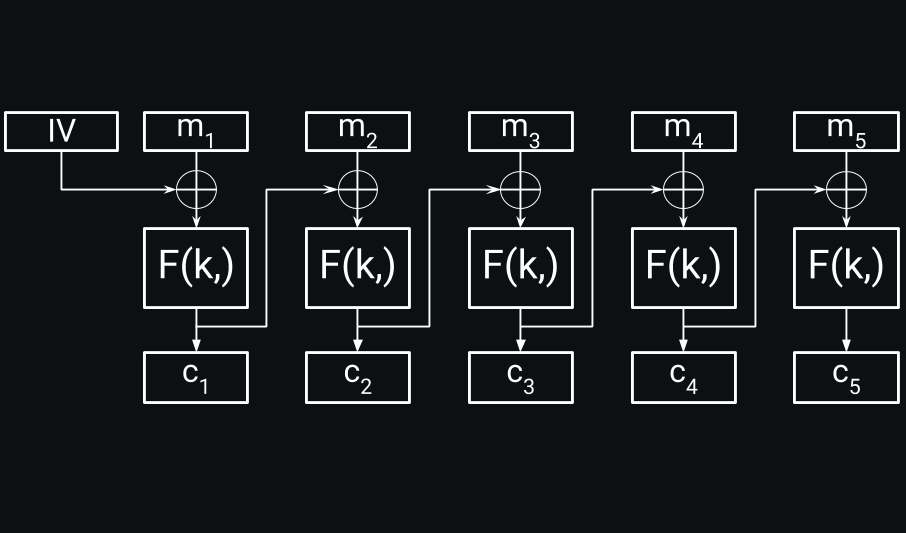
\includegraphics[width=0.9\textwidth]{CBC_1} 
	\end{figure}
\end{minipage}

\end{frame}

\begin{frame}{Padding}
\Large
\begin{center}
What if $\mathbf{m} = (m_1, m_2, ...)$ is not a multiple of the block length?
\end{center}
Example of {\color{Orange} bad} padding: filling up with $0'$s.
\[m = (\star \star \star  )\] 
that has length $<$ block length. Padding of such message:
\[m_{\text{padded}}=(\star \star \star  \; 0 \ldots 0  ) \]. Then for another message $m'$:
\[S(k,m_{\text{padded}}) = S(k, m'=(\star \star \star  \; 0 \ldots 0  ))\]
For any $m$, $S(m)=S(m||0)$.

\pause
\vspace{10pt}
\LARGE \centering
For $\mathbf{m} \neq \mathbf{m'}$ we want $\mathbf{m}||\text{pad} \neq \mathbf{m'}||\text{pad}$. In particular, padding must be $1 \leftrightarrow 1$.
	
\end{frame}

\begin{frame}{Padding}
	\Large
	\begin{enumerate}
		\itemsep1em
		\item {\color{Orange} ISO.} Pad with $10\ldots0$. `1' indicates beginning of the padding. \\
		Add a dummy block if $|m| < $ block length
		\pause 
		\item {\color{Orange} NIST, GOST}  
		\begin{figure}
			\captionsetup[subfigure]{labelformat=empty}
			%\centering
			%\stackunder[5pt]{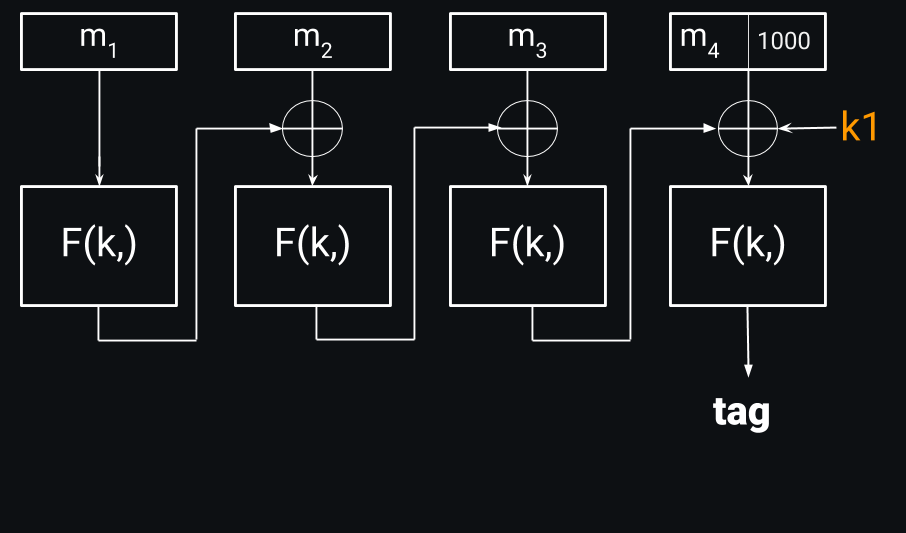
\includegraphics[width=.47\textwidth]{CBC_Mac_Padding}}{MRI-CGCM3}
			%\stackunder[5pt]{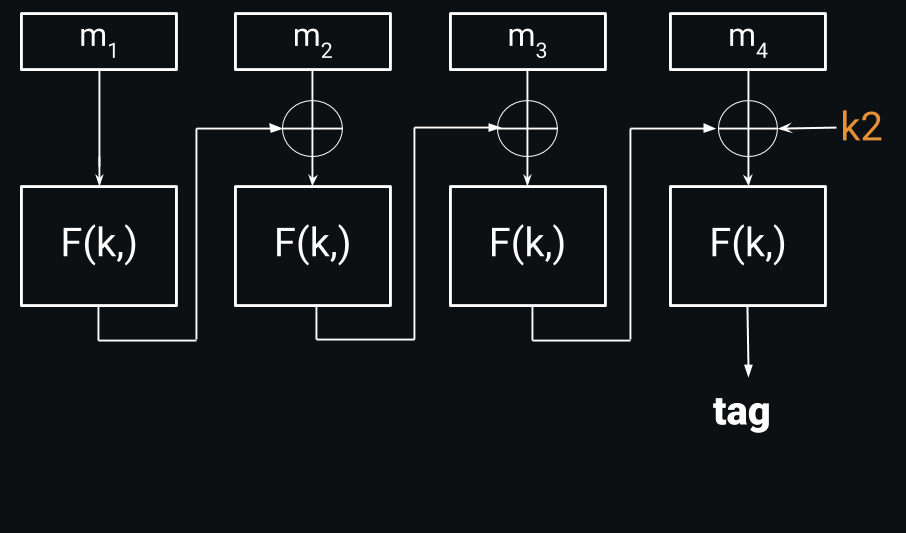
\includegraphics[width=.47\textwidth]{CBC_Mac_Padding_1}}{NorESM1-M}
			\begin{subfigure}{.5\textwidth}
				\centering
				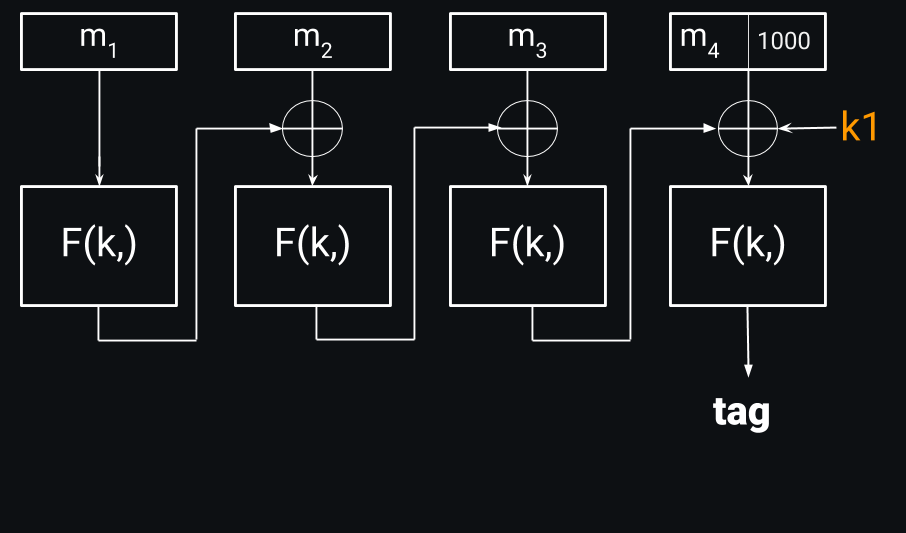
\includegraphics[width=.98\textwidth]{CBC_Mac_Padding}
				\caption{$m_4$< block-length}
			\end{subfigure}%
		 \begin{subfigure}{.5\textwidth}
			\centering
			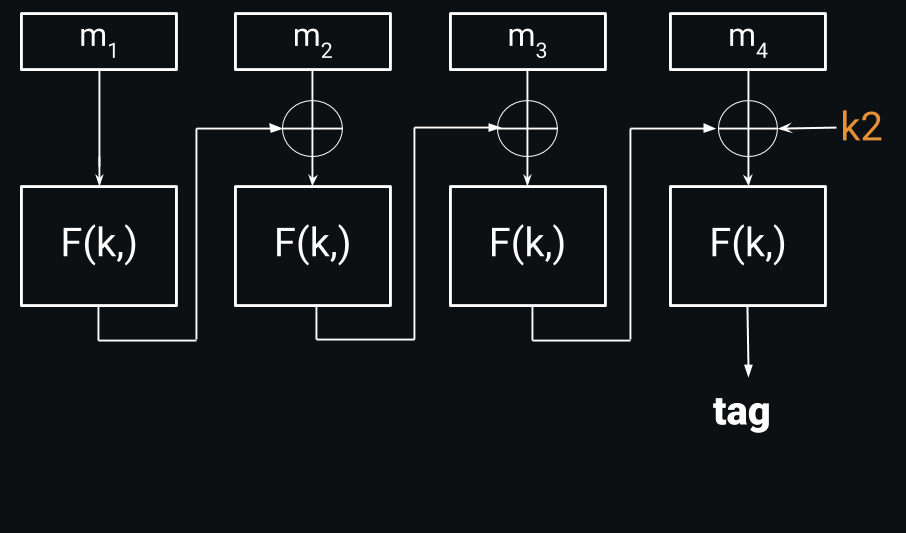
\includegraphics[width=.98\textwidth]{CBC_Mac_Padding_1}
			\caption{$m_4$= block-length}
		\end{subfigure}%
		\end{figure}
		\vspace{1em}
		Advantages: No dummy block, no additional application of $F$.
		 
	\end{enumerate}
\end{frame}

\begin{frame}{Some details on Programming Assignment 4}
\Large
Assume our tag is generated without the last encryption step for one-block message $m $ ($|m|=128$ bits).
\begin{figure}
	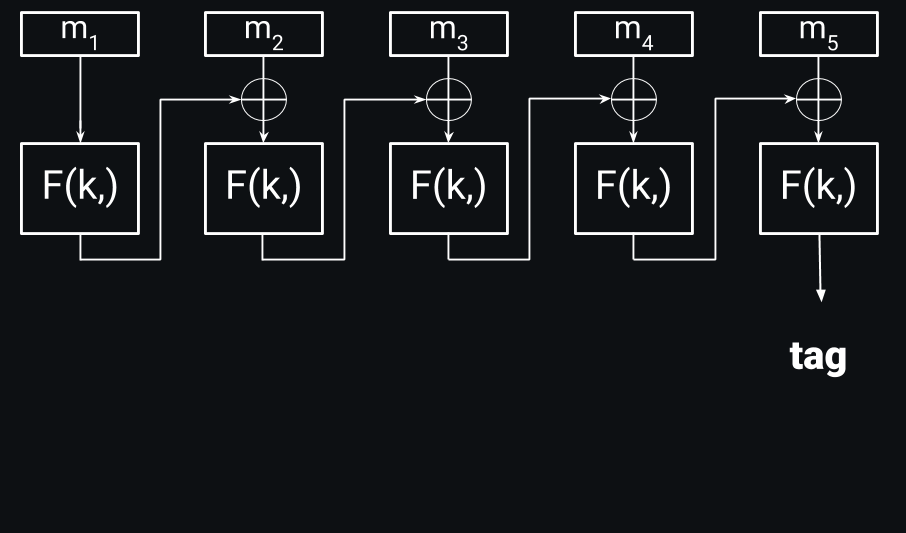
\includegraphics[width=0.8\textwidth]{Raw_CBC_Mac} 
\end{figure}

\vspace{-30pt}
Your task is to demonstrate an efficient tag forgery for such construction: by having $(m,t)$ - a valid (message, tag) pair, provide another valid pair $(m', t)$. \\
\emph{Hint:} $m'$ might consist of two blocks.
	
\end{frame}

\begin{frame}{Concluding slide}
\LARGE
	\begin{enumerate}
		\itemsep 1em
		\item Other types of MACs exist: Parallel Mac (PMAC), One-time MAC
		\item MACs are not Checksums! MACs {\color{Orange} require} secret keys
		\item DO NOT follow the Russian Wikipedia article on MACs
		\item For Russian project follow GOST'15 guidelines (link is on the course's webpage)
	\end{enumerate}
\vspace{10pt}
Next time: Message integrity with cryptographic hash functions
\end{frame}

\end{document}